%%%%%%%%%%%%%%%%%%%%%%%%%%%%%%%%%%%%%%%%%%%%%%%%%%%%%%%%%%%%%%%%%%%%%%%%%
%  Content: Main file of thesis template (master/enginering).
%  Author: Tomasz Kubik <tomasz.kubik@pwr.edu.pl>
%  Data: 1 marca 2020
%  Wersja: 0.4
%%%%%%%%%%%%%%%%%%%%%%%%%%%%%%%%%%%%%%%%%%%%%%%%%%%%%%%%%%%%%%%%%%%%%%%%%

\documentclass[a4paper,onecolumn,oneside,12pt,extrafontsizes]{memoir}
% In oder to prepare the manuscript for archives (2x1, double printed) you can:
% a) produce normal pdf, then convert it to pdf with two pages on one phisical page (solution suggested)
%
%   This can be done by:
%   - printing from Adobe Acrobat Reader with option "Multiple"
%   - using psutils
%
%      Windows (assuming that you have MiKTeX installed with the package pakiet miktex-psutils-bin-x64-2.9):
%        "c:\Program Files\MiKTeX 2.9\miktex\bin\x64\pdf2ps.exe" Dyplom.pdf Dyplom.ps
%        "c:\Program Files\MiKTeX 2.9\miktex\bin\x64\psnup.exe" -2 Dyplom.ps Dyplom2.ps
%        "c:\Program Files\MiKTeX 2.9\miktex\bin\x64\ps2pdf.exe" Dyplom2.ps Dyplom2.pdf
%        Del Dyplom2.ps Dyplom.ps
%
%     Linux:
%        pdf2ps Dyplom.pdf - | psnup -2 | ps2pdf - Dyplom2.pdf
%
%
% b) produce 'reduced' pdf by settning smaller fonts in the document class definition (it changes the formating thus it is not suggested)
%
%   Use of the following commands instead of original one:
%   \documentclass[a4paper,onecolumn,twoside,10pt]{memoir} 
%   \renewcommand{\normalsize}{\fontsize{8pt}{10pt}\selectfont}

%\usepackage[cp1250]{inputenc} % for cp1250 file encoding
\usepackage[utf8]{inputenc} % for UTF8 file encoding
\usepackage[T1]{fontenc}
\usepackage[polish,english]{babel}
%\usepackage[english]{babel}
%\DisemulatePackage{setspace}
\usepackage{setspace}
\usepackage{tabularx}
\usepackage{color,calc}
%\usepackage{soul} % packege with commands for text highliting
\usepackage{todonotes}
\usepackage{ebgaramond} % package with garamond font (required on the title page)

% Added by me during writing
% ==========================================================================
\usepackage{dirtree}    % simple directory tree for the an appendix
\usepackage{float}  %%  used for \begin{figure}[H]  <- insert exactly HERE!
\usepackage{caption} % used for adding source to an img
\newcommand{\source}[1]{\caption*{Source: {#1}} }

\usepackage{amsfonts}   % for mathbb



% for FSharp syntax
\usepackage{listings}
\usepackage{color}
\definecolor{bluekeywords}{rgb}{0.13,0.13,1}
\definecolor{greencomments}{rgb}{0,0.5,0}
\definecolor{redstrings}{rgb}{0.9,0,0}
\usepackage{upquote}
\lstdefinelanguage{FSharp}%
{morekeywords={let, new, match, with, rec, open, module, namespace, type, of, member, % 
and, for, while, true, false, in, do, begin, end, fun, function, return, yield, try, %
mutable, if, then, else, cloud, async, static, use, abstract, interface, inherit, finally },
  otherkeywords={ let!, return!, do!, yield!, use!, var, from, select, where, order, by },
  keywordstyle=\color{bluekeywords},
  sensitive=true,
  basicstyle=\ttfamily,
	breaklines=true,
  xleftmargin=\parindent,
  aboveskip=\bigskipamount,
	tabsize=4,
  morecomment=[l][\color{greencomments}]{///},
  morecomment=[l][\color{greencomments}]{//},
  morecomment=[s][\color{greencomments}]{{(*}{*)}},
  morestring=[b]",
  showstringspaces=false,
  literate={`}{\`}1,
  stringstyle=\color{redstrings},
}



% For C# syntax v1
% \usepackage{etoolbox}
% \usepackage{color}

% \definecolor{base0}{RGB}{131,148,150}
% \definecolor{base01}{RGB}{88,110,117}
% \definecolor{base2}{RGB}{238,232,213}
% \definecolor{sgreen}{RGB}{133,153,0}
% \definecolor{sblue}{RGB}{38,138,210}
% \definecolor{scyan}{RGB}{42,161,151}
% \definecolor{smagenta}{RGB}{211,54,130}

% \newcommand\digitstyle{\color{smagenta}}
% \newcommand\symbolstyle{\color{base01}}
% \makeatletter
% \newcommand{\ProcessDigit}[1]
% {%
%   \ifnum\lst@mode=\lst@Pmode\relax%
%   {\digitstyle #1}%
%   \else
%     #1%
%   \fi
% }
% \makeatother

% \lstdefinestyle{solarizedcsharp} {
%   language=[Sharp]C,
%   frame=lr,
%   linewidth=160mm,
%   breaklines=true,
%   tabsize=2,
%   numbers=left,
%   numbersep=5pt,
%   firstnumber=auto,
%   numberstyle=\tiny\ttfamily\color{base0},
%   rulecolor=\color{base2},
%   basicstyle=\footnotesize\ttfamily,
%   commentstyle=\color{base01},
%   morecomment=[s][\color{base01}]{/*+}{*/},
%   morecomment=[s][\color{base01}]{/*-}{*/},
%   morekeywords={  abstract, event, new, struct,
%                 as, explicit, null, switch,
%                 base, extern, object, this,
%                 bool, false, operator, throw,
%                 break, finally, out, true,
%                 byte, fixed, override, try,
%                 case, float, params, typeof,
%                 catch, for, private, uint,
%                 char, foreach, protected, ulong,
%                 checked, goto, public, unchecked,
%                 class, if, readonly, unsafe,
%                 const, implicit, ref, ushort,
%                 continue, in, return, using,
%                 decimal, int, sbyte, virtual,
%                 default, interface, sealed, volatile,
%                 delegate, internal, short, void,
%                 do, is, sizeof, while,
%                 double, lock, stackalloc,
%                 else, long, static,
%                 enum, namespace, string, var},
%   keywordstyle=\bfseries\color{sgreen},
%   showstringspaces=false,
%   stringstyle=\color{scyan},
%   identifierstyle=\color{sblue},
%   extendedchars=true,
%   literate=
%     {0}{{{\ProcessDigit{0}}}}1
%     {1}{{{\ProcessDigit{1}}}}1
%     {2}{{{\ProcessDigit{2}}}}1
%     {3}{{{\ProcessDigit{3}}}}1
%     {4}{{{\ProcessDigit{4}}}}1
%     {5}{{{\ProcessDigit{5}}}}1
%     {6}{{{\ProcessDigit{6}}}}1
%     {7}{{{\ProcessDigit{7}}}}1
%     {8}{{{\ProcessDigit{8}}}}1
%     {9}{{{\ProcessDigit{9}}}}1
%     {\}}{{\symbolstyle{\}}}}1
%     {\{}{{\symbolstyle{\{}}}1
%     {(}{{\symbolstyle{(}}}1
%     {)}{{\symbolstyle{)}}}1
%     {=}{{\symbolstyle{$=$}}}1
%     {;}{{\symbolstyle{$;$}}}1
%     {>}{{\symbolstyle{$>$}}}1
%     {<}{{\symbolstyle{$<$}}}1
%     {\%}{{\symbolstyle{$\%$}}}1,
% }

% \lstset{escapechar=@,style=solarizedcsharp}


% For C# syntax v12
\usepackage[T1]{fontenc}
\usepackage[scaled]{beramono}

\usepackage{color}
\definecolor{bluekeywords}{rgb}{0.13,0.13,1}
\definecolor{greencomments}{rgb}{0,0.5,0}
\definecolor{redstrings}{rgb}{0.9,0,0}

\usepackage{listings}
\lstset{language=[Sharp]C,
showspaces=false,
showtabs=false,
breaklines=true,
showstringspaces=false,
breakatwhitespace=true,
escapeinside={(*@}{@*)},
commentstyle=\color{greencomments},
keywordstyle=\color{bluekeywords}\bfseries,
stringstyle=\color{redstrings},
basicstyle=\ttfamily
}




%% Accorging to the rules the main font of the thesis should be Times.
%% In order to achieve it we use tgtermes font that offers shapes: normal, bold, italic, italic bold.
%% There is no slanted shape.
%% If you use slanted font in the text (typing \textsl{} commnand), then LaTeX will substitute it with a standard font giving you a warning.
%% Additionally tgtermes works for the running text. All maths (formulas, equations) will be rendered with a default font for math.
%% If you with to change the font for math, you must to do it yourself.

%% After installation of tgtermes package there might be a need to update font and mapping information 
%% This can be don by running the following commands (as administrator)
%% initexmf --admin --update-fndb
%% initexmf --admin --mkmaps

\usepackage{tgtermes}   
\renewcommand*\ttdefault{txtt}

% The settings regarding fonts were used in the earlier version of the template. It is kept for historical reasons
%\usepackage{mathptmx} 
%\usepackage{newtxtext,newtxmath} 
%\usepackage{newtxmath,tgtermes} 

\usepackage{listings} % used to render the source code 
% In UTF8 encoding there was a need to define the following mapping (otherwise the national characters were not recognized correctly)
%%\lstset{literate=%-
%%{ą}{{\k{a}}}1 {ć}{{\'c}}1 {ę}{{\k{e}}}1 {ł}{{\l{}}}1 {ń}{{\'n}}1 {ó}{{\'o}}1 {ś}{{\'s}}1 {ż}{{\.z}}1 {ź}{{\'z}}1 {Ą}{{\k{A}}}1 {Ć}{{\'C}}1 {Ę}{{\k{E}}}1 {Ł}{{\L{}}}1 {Ń}{{\'N}}1 {Ó}{{\'O}}1 {Ś}{{\'S}}1 {Ż}{{\.Z}}1 {Ź}{{\'Z}}1 
    %%{Ö}{{\"O}}1
    %%{Ä}{{\"A}}1
    %%{Ü}{{\"U}}1
    %%{ß}{{\ss}}1
    %%{ü}{{\"u}}1
    %%{ä}{{\"a}}1
    %%{ö}{{\"o}}1
    %%{~}{{\textasciitilde}}1
		%%{—}{{{\textemdash} }}1
%%}%{\ \ }{{\ }}1}

\newcommand{\listingcaption}[1]% added to handle captions of listings in two columns 
{%
\vspace*{\abovecaptionskip}\small 
\refstepcounter{lstlisting}\hfill%
Listing \thelstlisting: #1\hfill%\hfill%
\addcontentsline{lol}{lstlisting}{\protect\numberline{\thelstlisting}#1}
}%

% code style with line numbering (but these are commented out)
\lstset{
  %%basicstyle=\footnotesize\ttfamily,
  %%columns=fullflexible,
	%%showstringspaces=false,
	%%showspaces=false,
  breaklines=true,
  postbreak=\mbox{\textcolor{red}{$\hookrightarrow$}\space},
  %%numbers=left,
  %%firstnumber=1,
  %%numberfirstline=true,
	%%xleftmargin=17pt,
  %%framexleftmargin=17pt,
  %%framexrightmargin=5pt,
  %%framexbottommargin=4pt,
	belowskip=.5\baselineskip
}

% code style without line numbering
%%\lstset{
  %%basicstyle=\footnotesize\ttfamily,
  %%columns=fullflexible,
	%%showstringspaces=false,
	%%showspaces=false,
  %%breaklines=true,
  %%postbreak=\mbox{\textcolor{red}{$\hookrightarrow$}\space},
%%}

%% Here you have another example of code styling
%%\lstloadlanguages{% Check Dokumentation for further languages ...
%%C,
%%C++,
%%csh,
%%Java
%%}
%%
%%\definecolor{red}{rgb}{0.6,0,0} % for strings
%%\definecolor{blue}{rgb}{0,0,0.6}
%%\definecolor{green}{rgb}{0,0.8,0}
%%\definecolor{cyan}{rgb}{0.0,0.6,0.6}
%%
%%\lstdefinestyle{sqlstyle}{
%%language=SQL,
%%basicstyle=\footnotesize\ttfamily, 
%%numbers=left, 
%%numberstyle=\tiny, 
%%numbersep=5pt, 
%%tabsize=2, 
%%extendedchars=true, 
%%breaklines=true, 
%%showspaces=false, 
%%showtabs=true, 
%%xleftmargin=17pt,
%%framexleftmargin=17pt,
%%framexrightmargin=5pt,
%%framexbottommargin=4pt,
%%keywordstyle=\color{blue}, 
%%commentstyle=\color{green}, 
%%stringstyle=\color{red}, 
%%}
%%
%%\lstdefinestyle{sharpcstyle}{
%%language=[Sharp]C,
%%basicstyle=\footnotesize\ttfamily, 
%%numbers=left, 
%%numberstyle=\tiny, 
%%numbersep=5pt, 
%%tabsize=2, 
%%extendedchars=true, 
%%breaklines=true, 
%%showspaces=false, 
%%showtabs=true, 
%%xleftmargin=17pt,
%%framexleftmargin=17pt,
%%framexrightmargin=5pt,
%%framexbottommargin=4pt,
%%morecomment=[l]{//}, %use comment-line-style!
%%morecomment=[s]{/*}{*/}, %for multiline comments
%%showstringspaces=false, 
%%morekeywords={  abstract, event, new, struct,
                %%as, explicit, null, switch,
                %%base, extern, object, this,
                %%bool, false, operator, throw,
                %%break, finally, out, true,
                %%byte, fixed, override, try,
                %%case, float, params, typeof,
                %%catch, for, private, uint,
                %%char, foreach, protected, ulong,
                %%checked, goto, public, unchecked,
                %%class, if, readonly, unsafe,
                %%const, implicit, ref, ushort,
                %%continue, in, return, using,
                %%decimal, int, sbyte, virtual,
                %%default, interface, sealed, volatile,
                %%delegate, internal, short, void,
                %%do, is, sizeof, while,
                %%double, lock, stackalloc,
                %%else, long, static,
                %%enum, namespace, string},
%%keywordstyle=\color{cyan},
%%identifierstyle=\color{red},
%%stringstyle=\color{blue}, 
%%commentstyle=\color{green},
%%}


\renewcommand\lstlistlistingname{List of listings}
\makeatletter
%\renewcommand*{\l@lstlisting}[2]{\@dottedtocline{1}{0em}{2.3em}{#1}{#2}}
\g@addto@macro\insertchapterspace{\addtocontents{lol}{\protect\addvspace{10pt}}}
\renewcommand*{\l@lstlisting}{\@dottedtocline{1}{0em}{2.3em}}
\makeatother

\renewcommand*{\lstlistlistingname}{List of listings} \newlistof{lstlistoflistings}{lol}{\lstlistlistingname}



% It is possible to use packages mentioned below for making various tables but it is suggested to left them unused
%\usepackage{longtable}
%\usepackage{ltxtable}
%\usepackage{tabulary}

%%%%%%%%%%%%%%%%%%%%%%%%%%%%%%%%%%%%%%%%%%%%%%%%%%%
%% Settings related to the autmatic document typesetting
%% and floats placements
%%%%%%%%%%%%%%%%%%%%%%%%%%%%%%%%%%%%%%%%%%%%%%%%%%%
%\hyphenpenalty=10000		% do not break words too often
\clubpenalty=10000      % penalty for orphans
\widowpenalty=10000  % do not left widows
%\brokenpenalty=10000		% dont break words between pages - commented out because interfere with line breaking in lstlisting
%\exhyphenpenalty=999999		% dont break word with dash - commented out because interfere with line breaking in lstlisting
\righthyphenmin=3			% break at min 3 characters

%\tolerance=4500
%\pretolerance=250
%\hfuzz=1.5pt
%\hbadness=1450

\renewcommand{\topfraction}{0.95}
\renewcommand{\bottomfraction}{0.95}
\renewcommand{\textfraction}{0.05}
\renewcommand{\floatpagefraction}{0.35}

%%%%%%%%%%%%%%%%%%%%%%%%%%%%%%%%%%%%%%%%%%%%%%%%%%%
%%  Size settings: text, header and footer, marigins
%%  for documents based on memoir class
%%%%%%%%%%%%%%%%%%%%%%%%%%%%%%%%%%%%%%%%%%%%%%%%%%%
\setlength{\headsep}{10pt} 
\setlength{\headheight}{13.6pt} % baselineskip for 11pt font, i.e. \small, equals 13.6pt
\setlength{\footskip}{\headsep+\headheight}
\setlength{\uppermargin}{\headheight+\headsep+1cm}
\setlength{\textheight}{\paperheight-\uppermargin-\footskip-1.5cm}
\setlength{\textwidth}{\paperwidth-5cm}
\setlength{\spinemargin}{2.5cm}
\setlength{\foremargin}{2.5cm}
\setlength{\marginparsep}{2mm}
\setlength{\marginparwidth}{2.3mm}
%\settrimmedsize{297mm}{210mm}{*}
%\settrims{0mm}{0mm}	
\checkandfixthelayout[fixed] % needed to fix the layout
%%%%%%%%%%%%%%%%%%%%%%%%%%%%%%%%%%%%%%%%%%%%%%%%
%%  Settings related to the interline spaces, indentations, distances
%%%%%%%%%%%%%%%%%%%%%%%%%%%%%%%%%%%%%%%%%%%%%%%%
\linespread{1}
%\linespread{1.241}
\setlength{\parindent}{14.5pt}
%\setlength{\cftbeforechapterskip}{0.3em} % spaces in the table of contents
%\setbeforesecskip{10pt plus 0.5ex}%{-3.5ex \@plus -1ex \@minus -.2ex}
%\setaftersecskip{10pt plus 0.5ex}%\onelineskip}
%\setbeforesubsecskip{8pt plus 0.5ex}%{-3.5ex \@plus -1ex \@minus -.2ex}
%\setaftersubsecskip{8pt plus 0.5ex}%\onelineskip}
%\setlength\floatsep{6pt plus 2pt minus 2pt} 
%\setlength\intextsep{12pt plus 2pt minus 2pt} 
%\setlength\textfloatsep{12pt plus 2pt minus 2pt} 

%%%%%%%%%%%%%%%%%%%%%%%%%%%%%%%%%%%%%%%%%%%%%%%%%%%
%%  Pakiety i komendy zastosowane tylko do zamieszczenia informacji o użytych komendach i fontach
%%  Normalnie nie są potrzebne, można je zamarkować podczas redakcji pracy
%%%%%%%%%%%%%%%%%%%%%%%%%%%%%%%%%%%%%%%%%%%%%%%%%%%
\usepackage{memlays}     % extra layout diagrams, used only in template for 'debugging'. Is uses layouts package. Comment out them both if you edit your thesis
%\usepackage{layouts}
\usepackage{printlen} % allows displeying the values of defined lengths, used onlu in template for 'debugging'. Comment out it if you edit your thesis
\uselengthunit{pt}
\makeatletter
\newcommand{\showFontSize}{\f@size pt} % makro wypisujące wielkość bieżącej czcionki
\makeatother
% if you wish to show the frames:
%\usepackage{showframe} 


%%%%%%%%%%%%%%%%%%%%%%%%%%%%%%%%%%%%%%%%%%%%%%%%%%%
%%  Enumerated lists definitions
%%%%%%%%%%%%%%%%%%%%%%%%%%%%%%%%%%%%%%%%%%%%%%%%%%%

% Item lists have, by default, the bullets which are charactes not existing in the set of tgtermes fonts
% Therefore these are substituted by LaTeX with characters from standard set of fonts. In order to change this
% behavior you cad declare substitutions as below
%    \DeclareTextCommandDefault{\textbullet}{\ensuremath{\bullet}}
%    \DeclareTextCommandDefault{\textasteriskcentered}{\ensuremath{\ast}}
%    \DeclareTextCommandDefault{\textperiodcentered}{\ensuremath{\cdot}}
% But the better way is to redefine enumitem environment from enumitem package
\usepackage{enumitem}
\setlist{noitemsep,topsep=4pt,parsep=0pt,partopsep=4pt,leftmargin=*} % this makes list more compact
\setenumerate{labelindent=0pt,itemindent=0pt,leftmargin=!,label=\arabic*.} % it is possible to use \arabic or \alph, if the enumerations are supposed to be rendered with different numbers
\setlistdepth{4} % limits the depth of nested enumeration
\setlist[itemize,1]{label=$\bullet$}  % here we define the bullet at each of the levels
\setlist[itemize,2]{label=\normalfont\bfseries\textendash}
\setlist[itemize,3]{label=$\ast$}
\setlist[itemize,4]{label=$\cdot$}
\renewlist{itemize}{itemize}{4}

%%%http://tex.stackexchange.com/questions/29322/how-to-make-enumerate-items-align-at-left-margin
%\renewenvironment{enumerate}
%{
%\begin{list}{\arabic{enumi}.}
%{
%\usecounter{enumi}
%%\setlength{\itemindent}{0pt}
%%\setlength{\leftmargin}{1.8em}%{2zw} % 
%%\setlength{\rightmargin}{0zw} %
%%\setlength{\labelsep}{1zw} %
%%\setlength{\labelwidth}{3zw} % 
%\setlength{\topsep}{6pt}%
%\setlength{\partopsep}{0pt}%
%\setlength{\parskip}{0pt}%
%\setlength{\parsep}{0em} % 
%\setlength{\itemsep}{0em} % 
%%\setlength{\listparindent}{1zw} % 
%}
%}{
%\end{list}
%}

\makeatletter
\renewenvironment{quote}{
	\begin{list}{}
	{
	\setlength{\leftmargin}{1em}
	\setlength{\topsep}{0pt}%
	\setlength{\partopsep}{0pt}%
	\setlength{\parskip}{0pt}%
	\setlength{\parsep}{0pt}%
	\setlength{\itemsep}{0pt}
	}
	}{
	\end{list}}
\makeatother

%%%%%%%%%%%%%%%%%%%%%%%%%%%%%%%%%%%%%%%%%
%%  Package for index generation (must be set before hyperref)
%%%%%%%%%%%%%%%%%%%%%%%%%%%%%%%%%%%%%%%%%
%%\DisemulatePackage{imakeidx} % uncomment it out if you wish to generate an index
%%\usepackage[makeindex,noautomatic]{imakeidx} % here we say that the index can not be generated automatically

\makeatletter
%%%\renewenvironment{theindex}
							 %%%{\vskip 10pt\@makeschapterhead{\indexname}\vskip -3pt%
								%%%\@mkboth{\MakeUppercase\indexname}%
												%%%{\MakeUppercase\indexname}%
								%%%\vspace{-3.2mm}\parindent\z@%
								%%%\renewcommand\subitem{\par\hangindent 16\p@ \hspace*{0\p@}}%%
								%%%\phantomsection%
								%%%\begin{multicols}{2}
								%%%%\thispagestyle{plain}
								%%%\parindent\z@                
								%%%%\parskip\z@ \@plus .3\p@\relax
								%%%\let\item\@idxitem}
							 %%%{\end{multicols}\clearpage}
%%%
\makeatother


\usepackage{ifpdf}
\newif\ifpdf \ifx\pdfoutput\undefined
\pdffalse % we are not running PDFLaTeX
\else
\pdfoutput=1 % we are running PDFLaTeX
\pdftrue \fi
\ifpdf
    \usepackage[pdftex,bookmarks,breaklinks,unicode]{hyperref}
    \usepackage[pdftex]{graphicx}
    \DeclareGraphicsExtensions{.pdf,.jpg,.mps,.png}
    \pdfcompresslevel=9
    \pdfoutput=1
    \makeatletter
    \AtBeginDocument{  % Here are the metadata that will be embedded in the resulting pdf. Please fill in them correctly
    \hypersetup{
        pdfinfo={
        Title = {\@title},
        Author = {\@author},
        Subject={},
        Keywords={},  
		Producer={},
		Creator={pdftex}
	}}
    }
    \pdftrailerid{} %Remove ID
    \pdfsuppressptexinfo15 %Suppress PTEX.Fullbanner and info of imported PDFs

    \makeatother
\else
    \usepackage{graphicx}
    \DeclareGraphicsExtensions{.eps,.ps,.jpg,.mps,.png}
\fi

\sloppy

%\graphicspath{{figures01/}{figures02/}} %% if you with to have set the paths to figures  


% Depth of numbering
\setcounter{secnumdepth}{2}
\setcounter{tocdepth}{2}
\setsecnumdepth{subsection} % activating subsubsec numbering in doc


% dots aftes sections numbers
\makeatletter
\def\@seccntformat#1{\csname the#1\endcsname.\quad}
\def\numberline#1{\hb@xt@\@tempdima{#1\if&#1&\else.\fi\hfil}}
\makeatother

\renewcommand{\chapternumberline}[1]{#1.\quad}
\renewcommand{\cftchapterdotsep}{\cftdotsep}

%\definecolor{niceblue}{rgb}{.168,.234,.671}

% Fonts in figures and tables captions
\captionnamefont{\small}
\captiontitlefont{\small}
% macro adjusting the way the chapter title is rendered
%\def\printchaptertitle##1{\fonttitle \space \thechapter.\space ##1} 

%\usepackage{ltcaption}
% The ltcaption package supports \CaptionLabelFont & \CaptionTextFont introduced by the NTG document classes
%\renewcommand\CaptionLabelFont{\small}
%\renewcommand\CaptionTextFont{\small}

% Redefinitions of labels for tables, figures and bibliography 
%\AtBeginDocument{% 
%        \addto\captionspolish{% 
%        \renewcommand{\tablename}{Tab.}% 
%}%} 

%\AtBeginDocument{% 
%        \addto\captionspolish{% 
%        \renewcommand{\chaptername}{Rozdział}% 
%}} 

%\AtBeginDocument{% 
%        \addto\captionspolish{% 
%        \renewcommand{\figurename}{Rys.}% 
%}%}


%\AtBeginDocument{% 
%        \addto\captionspolish{% 
%        \renewcommand{\bibname}{Literatura}% 
%}%}

%\AtBeginDocument{% 
%        \addto\captionspolish{% 
%        \renewcommand{\listfigurename}{Spis rysunków kubaTest}% 
%}%}

%\AtBeginDocument{% 
%        \addto\captionspolish{% 
%        \renewcommand{\listtablename}{Spis tabel}% 
%}%}

%\AtBeginDocument{% 
%        \addto\captionspolish{% 
%\renewcommand\indexname{Indeks rzeczowy}
%}%}

%%%%%%%%%%%%%%%%%%%%%%%%%%%%%%%%%%%%%%%%%%%%%%%%%%%%%%%%%%%%%%%%%%                  
%% Definition of headers and footers appearing on pages
%%%%%%%%%%%%%%%%%%%%%%%%%%%%%%%%%%%%%%%%%%%%%%%%%%%%%%%%%%%%%%%%%%                  
\addtopsmarks{headings}{%
\nouppercaseheads % added at the beginning
}{%
\createmark{chapter}{both}{shownumber}{}{. \space}
%\createmark{chapter}{left}{shownumber}{}{. \space}
\createmark{section}{right}{shownumber}{}{. \space}
}%use the new settings

\makeatletter
\copypagestyle{outer}{headings}
\makeoddhead{outer}{}{}{\small\itshape\rightmark}
\makeevenhead{outer}{\small\itshape\leftmark}{}{}
\makeoddfoot{outer}{\small\@author:~\@titleShort}{}{\small\thepage}
\makeevenfoot{outer}{\small\thepage}{}{\small\@author:~\@title}
\makeheadrule{outer}{\linewidth}{\normalrulethickness}
\makefootrule{outer}{\linewidth}{\normalrulethickness}{2pt}
\makeatother

% fix plain
\copypagestyle{plain}{headings} % overwrite plain with outer
\makeoddhead{plain}{}{}{} % remove right header
\makeevenhead{plain}{}{}{} % remove left header
\makeevenfoot{plain}{}{}{}
\makeoddfoot{plain}{}{}{}

\copypagestyle{empty}{headings} % overwrite plain with outer
\makeoddhead{empty}{}{}{} % remove right header
\makeevenhead{empty}{}{}{} % remove left header
\makeevenfoot{empty}{}{}{}
\makeoddfoot{empty}{}{}{}


%%%%%%%%%%%%%%%%%%%%%%%%%%%%%%%%%%%%%%%
%% Definition of title page
%%%%%%%%%%%%%%%%%%%%%%%%%%%%%%%%%%%%%%%
\makeatletter
% University
\newcommand\uczelnia[1]{\renewcommand\@uczelnia{#1}}
\newcommand\@uczelnia{}
% Faculty
\newcommand\wydzial[1]{\renewcommand\@wydzial{#1}}
\newcommand\@wydzial{}
% Field
\newcommand\kierunek[1]{\renewcommand\@kierunek{#1}}
\newcommand\@kierunek{}
% Speciality
\newcommand\specjalnosc[1]{\renewcommand\@specjalnosc{#1}}
\newcommand\@specjalnosc{}
% Title in english
\newcommand\titleEN[1]{\renewcommand\@titleEN{#1}}
\newcommand\@titleEN{}
% Short title (used in headers/footers
\newcommand\titleShort[1]{\renewcommand\@titleShort{#1}}
\newcommand\@titleShort{}
% Supervisor
\newcommand\supervisor[1]{\renewcommand\@promotor{#1}}
\newcommand\@promotor{}

%\usepackage[absolute]{textpos} % not used because picture environment was applied

\def\maketitle{%
  \pagestyle{empty}%
%%\garamond 
	\fontfamily{\ebgaramond@family}\selectfont % title page must be typed in garamond font
%%%%%%%%%%%%%%%%%%%%%%%%%%%%%%%%%%%%%	
%% Below there is a declaration of picture including title and author text.
%% This text must be placed inside a 110mmx75mm window, whose upper left corner
%% is located at 77mm from the left and 111mm from the top of the page border
%% (the cover of the thesis has a window cutted in it just of this size). 
%% Plese check if the title and the author are really correclty placed.
%% In case of bad fitting please adjust attributes of the commands used
%% to put the window in a correct place.
%%
%% The color cover (with cutted window) should be available from administration
%% Please notice, that this cover is a bit bigger that A4 page by 3mm. Cutt these
%% margins to make the cover of the same size as the page
%%%%%%%%%%%%%%%%%%%%%%%%%%%%%%%%%%%%%	
\newlength{\tmpfboxrule}
\setlength{\tmpfboxrule}{\fboxrule}
\setlength{\fboxsep}{2mm}
\setlength{\fboxrule}{0mm} 
%\setlength{\fboxrule}{0.1mm} %% jeśli chcemy zobaczyć ramkę
\setlength{\unitlength}{1mm}
\begin{picture}(0,0)
\put(44,-129){\fbox{
\parbox[c][71mm][c]{104mm}{\centering%\lineskip=34pt 
\fontsize{16pt}{18pt}\selectfont \@titleEN\\[5mm]
\fontsize{16pt}{18pt}\selectfont \@title\\[15mm]
\fontsize{16pt}{18pt}\selectfont AUTHOR:\\[2mm]
\fontsize{14pt}{16pt}\selectfont \@author}
}
}
\end{picture}
\setlength{\fboxrule}{\tmpfboxrule} 
%%%%%%%%%%%%%%%%%%%%%%%%%%%%%%%%%%%%%
%% Reszta strony z nazwą uczelni, wydziału, kierunkiem, specjalnością
%% promotorem, oceną pracy, miastem i rokiem
	{\centering%\vspace{-1cm}
		{\fontsize{22pt}{24pt}\selectfont \@uczelnia}\\[0.4cm]
		{\fontsize{22pt}{24pt}\selectfont \@wydzial}\\[0.5cm]
		  \hrule %\vspace*{0.7cm}
	}
{\flushleft\fontsize{14pt}{16pt}\selectfont%
\begin{tabular}{ll}
FIELD: & \@kierunek\\
SPECIALIZATION: & \@specjalnosc\\
\end{tabular}\\[1.3cm]
}
{\centering
{\fontsize{32pt}{36pt}\selectfont ENGINEERING}\\[0.5cm]
{\fontsize{32pt}{36pt}\selectfont THESIS}\\[2.5cm]
}
\vfill
\begin{tabularx}{\linewidth}{p{6cm}l}
		&{\fontsize{16pt}{18pt}\selectfont SUPERVISOR:}\\[2mm] %UWAGA: tutaj jest miejsce na nazwisko promotora pracy
		&{\fontsize{14pt}{16pt}\selectfont \@promotor}\\[10mm]
		&{\fontsize{16pt}{18pt}\selectfont GRADE:}\\[20mm]
	\end{tabularx}
\vspace{2cm}
\hrule\vspace*{0.3cm}
{\centering
{\fontsize{16pt}{18pt}\selectfont \@date}\\[0cm]
}
%\ungaramond
\normalfont
 \cleardoublepage
}
\makeatother
%%%%%%%%%%%%%%%%%%%%%%%%%%%%%%%%%%%%%%%%%

%\AtBeginDocument{\addtocontents{toc}{\protect\thispagestyle{empty}}}




%%%%%%%%%%%%%%%%%%%%%%%%%%%%%%%%%%%%%%%%%
%%  Metadane dokumentu 
%%%%%%%%%%%%%%%%%%%%%%%%%%%%%%%%%%%%%%%%%
\title{Wykorzystanie programowania funkcyjnego do wyceny wybranych instrumentów finansowych}
\titleShort{Engineering thesis}
\titleEN{Use of functional programming in modeling selected financial instruments}
\author{Jakub Unold}
\uczelnia{WROCLAW UNIVERSITY OF SCIENCE AND TECHNOLOGY}
\wydzial{FACULTY OF ELECTRONICS}
\kierunek{AUTOMATICS AND ROBOTICS}
\specjalnosc{INDUSTRY 4.0}
\supervisor{Prof. Wojciech Bożejko, Ph.D., D.Sc., M.A.}
\date{WROCŁAW, 2020}

% Setting the space above nonnumbered chapters and list: ToC, LoT, LoF, Index
% Spis treści, Spis tabel, Spis rysunków, Indeks rzeczowy

%\newlength{\linespace}
%\setlength{\linespace}{-\beforechapskip-\topskip+\headheight+\topsep}
%\makechapterstyle{noNumbered}{%
%\renewcommand\chapterheadstart{\vspace*{\linespace}}
%}

%% powyższa komenda załatwia to, co robią komendy poniższe dla spisów
%\renewcommand*{\tocheadstart}{\vspace*{\linespace}}
%\renewcommand*{\lotheadstart}{\vspace*{\linespace}}
%\renewcommand*{\lofheadstart}{\vspace*{\linespace}}

%%%%%%%%%%%%%%%%%%%%%%%%%%%%%%%%%%%%%%%%%%%%%%%%%%%%%%%%%%%%%%
%                  Beginning of the document 
%%%%%%%%%%%%%%%%%%%%%%%%%%%%%%%%%%%%%%%%%%%%%%%%%%%%%%%%%%%%%%
%\includeonly{abbreviations,chapter01} % uncomment it if you with to complile only selected latex files (this will speed up compilation, especially if you focuse on a specific part of the thesis)

\begin{document}

\selectlanguage{english}

% Here you have the commands for setting the spacing (do not change)
%\SingleSpacing
%\OnehalfSpacing
%\DoubleSpacing

%\settypeoutlayoutunit{cm} % for debbuging
%\typeoutstandardlayout    % prints on stdout the info about settings
\pdfbookmark[0]{Title}{Tytul.1}
\maketitle

%% The information about licence given below can be safely commented out when editing the thesis (the licence covers the text with instructions on how to use the template, but not the template itself).
%\newpage
%\thispagestyle{empty}
%\mbox{}\vfill
%\noindent\begin{tabular}{@{}ll} Opracował: & Tomasz Kubik \texttt{<tomasz.kubik@pwr.edu.pl>}\\
% Data: & marzec 2020 
% \end{tabular}\\[15mm]
%\noindent
\includegraphics[width=3cm]{by-nc-sa}\newline
%{\normalfont 
%Tekst zawarty\todo{coś} w niniejszym szablonie jest udostępniany na licencji Creative Commons: \emph{Uznanie autorstwa %-- Użycie niekomercyjne -- Na tych samych warunkach, 3.0 Polska}, Wrocław 2020. \\[2pt]
%Oznacza to, że wszystkie przekazane treści można kopiować i  wykorzystywać do celów niekomercyjnych, a także tworzyć %na ich podstawie utwory zależne pod warunkiem podania autora i~nazwy licencjodawcy oraz udzielania na utwory zależne %takiej samej licencji. Tekst licencji jest dostępny pod adresem: %\url{http://creativecommons.org/licenses/by-nc-sa/3.0/pl/}.\\[2pt]
%Podczas redakcji pracy dyplomowej poniższą stronę można usunąć (CC dotyczy tekstu, a nie samego latexowego szablonu)
%}
%\newpage


\chapterstyle{noNumbered}  % Below there are declarations of various lists. Please comment out those which are too short (the list should contain at least 5 items)
\pagestyle{outer}
\mbox{}\pdfbookmark[0]{Table of contents}{spisTresci.1}
% \mbox{}\pdfbookmark[0]{Table of contents}{Table of contents.1}
\tableofcontents* 

%\newpage
%\mbox{}\pdfbookmark[0]{List of figures}{spisRysunkow.1}
%\addcontentsline{toc}{chapter}{Spis rysunków}
%\listoffigures*

%\newpage
%\mbox{}\pdfbookmark[0]{List of tables}{spisTabel.1}
%\addcontentsline{toc}{chapter}{Spis tabel}
%\listoftables*

%\newpage
%\mbox{}\pdfbookmark[0]{List of listings}{spisListingow.1}
%\addcontentsline{toc}{chapter}{Spis listingów}
%\lstlistoflistings*

% Below there are inclusions of latex files
\include{abbreviations} % If abbreviations list is short, you can comment it out
\chapterstyle{default}
% \chapter*{Abstract}%
\addcontentsline{toc}{chapter}{\numberline{}Abstract}%
    This paper is an overview of some methods used for pricing selected financial instruments (or their derivatives). The main part of the project was creating a tool - a computer program written mostly in F\# for that purpose. The application is named \textit{MARS App} -- it is an acronym  of the English words \textit{Market And Risk Simulation}. Two models have been presented: first being Black-Scholes model from 1973 which gives an estimate of the price of a European-style option. As the underlying asset a stock price was used. In order to generate stock prices over time Geometric Brownion Motion has been implemented as this stochastic process is usually applied in the Black-Scholes model. The other model is Black's model from 1976 which is a slightly altered Black-Scholes model while it is adjusted for valuing options on futures contracts.
    
    This paper can be as well a kind of a guide how to create an F\# application using MVVM architecture with XAML markup language for creating user interface as such tutorials are scarce in literature.
    
    \emph{Keywords: functional programming, financial instruments, pricing, MVVM, Black-Scholes, Black, Myron, Scholes, Geometric Brownian Motion, Random Walk, Standard Brownian Motion}

\chapter*{Streszczenie}%
\addcontentsline{toc}{chapter}{\numberline{}Streszczenie}%
    W prezentowanej pracy inżynierskiej przedstawiono proces tworzenia narzędzia do wyceny wybranych instrumentów finansowych. Zaprezentowano wycenę europejskiej opcji przy użyciu znanego modelu Blacka-Scholes'a z 1973 roku, gdzie instrumentem podstawowym jest akcja wygenerowana za pomocą Geometrycznego Ruchu Browna. Pokazano również zastosowanie modelu Black'a z 1976 roku, gdzie w przeciwieństwie do poprzedniego modelu cena instrumentu bazowego zostaje zastąpiona zdyskontowaną wartością kontraktu futures/forward na ten instrument.
    
    W tym celu została stworzona aplikacja desktopowa w języku F\#, w paradygmacie programowania funkcyjnego, przy użyciu wzorca MVVM oraz technologii XAML do stworzenia interfejsu użytkownika. Aplikacja nosi nazwę MARS App -- jest to akronim od angielskiego \textit{Market And Risk Simulation Application}, co oznacza aplikację przeznaczoną do symulacji rynku i ryzyka. Praca zawiera również swoisty poradnik, jak stworzyć aplikację w języku F\#, opartą o architekturę MVVM w zintegrowanym środowisku programistycznym Visual Studio 2019 będącym produktem firmy Microsoft. Powyższy stos technologiczny nie jest często spotykany, co przejawia się zredukowaną ilością poradników pomagających stworzyć podobną aplikację nowym użytkownikom.
    
    \emph{Słowa kluczowe: programowanie funkcyjne, instrumenty finansowe, wycena, MVVM, Black-Scholes, Black, Myron, Scholes, Geometryczny Ruch Browna, Błądzenie Losowe, Standardowy Ruch Browna}
\chapter{Introduction}
\section{Streszczenie}
    W poniższej pracy inżynierskiej przedstawiono proces tworzenia narzędzia do wyceny wybranych instrumentów finansowych. Zaprezentowano wycenę europejskiej opcji przy użyciu znanego modelu Blacka-Scholes'a z 1973 roku, gdzie instrumentem podstawowym jest akcja wygenerowana za pomocą Geometrycznego Rruchu Browna. Pokazano również zastosowanie modelu Black'a z 1976 roku, gdzie w przeciwieństwie do poprzedniego modelu cena instrumentu bazowego zostaje zastąpiona zdyskontowaną wartością kontraktu futures/forward na ten instrument.
    
    W tym celu została stworzona aplikacja desktopowa w języku F\#, w paradygmacie programowania funkcyjnego, przy użyciu wzorca MVVM oraz technologii XAML do stworzenia interfejsu użytkownika. Aplikacja nosi nazwę MARS App -- jest to akronim od angielskiego \textit{Market And Risk Simulation Application}, co oznacza aplikację przeznaczoną do symulacji rynku i ryzka. Praca zawiera również swoisty poradnik, jak stworzyć aplikację w języku F\#, opartą o architekturę MVVM w zintegrowanym środowisku programistycznym Visual Studio 2019 będącym produktem firmy Microsoft, ponieważ dokładnie powyższe połączenie różnych technologii nie jest bardzo często spotykane, co przejawia się zredukowaną ilością poradników pomagających stworzyć podobną aplikację nowym użytkownikom.
    
    \emph{Słowa kluczowe: programowanie funkcyjne, instrumenty finansowe, wycena, MVVM, Black-Scholes, Black}

\section{Abstract}
    This paper is an overview of some methods used for pricing selected financial instruments (or their derivatives). Main part of the project was creating a tool - computer program written mostly in F\# for that purpose. The application is named \textit{MARS App} -- it is an acronym  of the English words \textit{Market And Risk Simulation}. Two models have been presented: first being Black-Scholes model from 1973 which gives an estimate of the price of european-style option. As the underlying asset stock price was used. In order to generate stock prices over time Geometric Brownion Motion has been implemented as this stochastic process is usually applied in the Black-Scholes model. The other model is Black's model from 1976 which is a slightly altered Black-Scholes model while it is adjusted for valuing options on futures contracts.
    
    This paper can be as well kind of a guide how to create an F\# application using MVVM architecture with XAML markup language for creating user interface as such tutorials are scarce in literature.
    
    \emph{Keywords: functional programming, financial instruments, pricing, MVVM, Black-Scholes, Black}

\section{Thesis assumptions}
    The main goal is to create a tool in functional programming paradigm which will be used to price selected financial instruments. To achieve this goal F\# programming language will be used as it was created mostly to support functional programming.
    
    App will consist of several different technologies such as MVVM design pattern, XAML language to create View part of the project and minor C\# background to connect XAML's View with F\#'s ViewModel. Everything will be written in Visual Studio 2019 IDE.
    
    Basic assumptions within the application include:
    \begin{itemize}
    \item Ability to specialize the product (maturity date, strike price, underlying asset price).
    \item Implementing Black-Scholes model to price options.
    \todo{Add GBM}
    \todo{Add several greeks}
    \end{itemize}

\section{Scope of the thesis}
    \todo{fill in at the end}
    In chapter 1 - blabla
    In chapter 2 I will talk about blablah

\section{Technologies Overview}
\subsection{Programming paradigms}
    Programming paradigm is nothing more but an overall concept which describes \textit{how} the programming is done and what is the methodology behind the language that adheres to a specific type of a paradigm. Throughout the years programming languages evolved, new ones have been created, so that today there are from 150, according to TIOBE Programming Community, up to 700, listed by Wikipedia, different programming languages \cite{numberOfProgrammingLanguages}. Although some sources \cite{numberOfProgrammingLanguages_hopl_info} state that there are almost as many as 9000 (sic) programming languages the exact number of those is not that important -- rather variety and the fact that there are many of them is crucial as it indicates that they must differ from each other and it turns out these differences can somehow be grouped, what is presented below.
    
    The most basic and intuitive approach into dividing paradigms is into 2 groups:
    \begin{itemize}
        \item Imperative Programming
        \item Declarative Programming
    \end{itemize}
    
    \subsubsection{Imperative Programming}
    This way of programming is not by accident described as the first one -- historically languages that present this type of programming have emerged primarily. Imperative programming enables the programmer to manage processor's behaviour on much more precise level. Commands show step-by-step how the computation is executed. These commands affect a program's state. This paradigm focuses on describing \textit{how} the goal should be achieved.
    
    Imperative programming can be further broken down into 3 groups:
    \begin{enumerate}
        \item \textbf{Procedural Programming} -- underlying model is based on a procedure (set of coded instructions \cite{procedureDefinition}). It has the ability to reuse code written once. Examples of procedural programming languages:
            \begin{itemize}
                \item C
                \item C++
                \item Java
                \item ColdFusion
                \item Pascal
            \end{itemize}
        \item \textbf{Object Oriented Programming} -- program is a set of classes and objects (instances of a class) that are meant to interact with each other. Examples of languages supporting OOP paradigm:
            \begin{itemize}
                \item Objective-C
                \item C++
                \item Java
                \item Visual Basic .NET
                \item Python
            \end{itemize}
        \item \textbf{Parallel Processing Approach} -- this style of programming is designed to divide computing the code into multiple processors in order to minimize time required for computation. Example of languages supporting parallel programming approach:
            \begin{itemize}
                \item NESL
                \item C
                \item C++
            \end{itemize}
    \end{enumerate}
    
    \subsubsection{Declarative Programming}
    On the other hand a programmer may want to focus not on \textit{how} the code should be ran on a computer but rather what \textit{what the result should look like} and the way of obtaining it is not the most important thing. One would rather give it up to the compiler to decide what is the best way of achieving the result. Declarative programming is also consisted of smaller groups, such as:
    \begin{enumerate}
        \item \textbf{Logic Programming} -- in logic programming the programmer has a knowledge, expressed in a logical form, about facts and rules concerning specific problem \cite{logicProgramming}. This type of programming resembles a mathematical proof. \textbf{Prolog} language is an example of this programming paradigm.
        
        \item \textbf{Database-Driven Programming Approach} -- it is based on storing the data and moving it, as well as the keeping information about relations between entities. \textbf{SQL} is one of the most popular examples of this programming group.
        
        \item \textbf{Functional Programming} -- like object in object-related programming in functional programming the most basic unit is a function. Shared state is avoided, as well as mutable data (the programmer is unable to crate a variable). Examples of functional programming paradigm:
            \begin{itemize}
                \item F\#
                \item Haskell
                \item Common Lisp
                \item OCaml
                \item Racket
            \end{itemize}
    \end{enumerate}

\subsection{F\#}
    F\# is a programming language that was created back in 2005 by Don Syme in cooperation with Microsoft Research. Although it is multi-paradigm programming language it best fits the functional, declarative programming group. It is open-source and belongs to .NET Framework \cite{WhatIsFSharp} \cite{FSharpWiki}.
    
    F\# is strongly typed language that uses type interference. It has lightweight syntax and is immutable by default. Lightweight syntax can be observed in low signal-to-noise ratio in comparison to other languages (for example C\#).
    
    \begin{lstlisting}[caption=C\# code example]
        public static class SumOfSquaresHelper
        {
           public static int Square(int i)
           {
              return i * i;
           }
    
           public static int SumOfSquares(int n)
           {
              int sum = 0;
              for (int i = 1; i <= n; i++)
              {
                 sum += Square(i);
              }
              return sum;
           }
        }
        
        int r = SumOfSquaresHelper.SumOfSquares(100);
    \end{lstlisting}
    
    \begin{lstlisting}[language=FSharp, caption=F\# code example]
        let sumOfSquares n = 
           [1..10] |> List.map (fun x -> x*x) |> List.sum
        
        let r = sumOfSquares 100
    \end{lstlisting}
    
    Both above snippets are taken from the site \url{https://fsharpforfunandprofit.com/} with minor changes applied to further improve F\# code by using lambda function \cite{compareCandF}. Both of these perform the same task -- count the sum of squares of all integers preceding certain number. The goal is to show how succinct F\# can be in comparison to the same code but written in C\#.
    
    Taking all F\# features into account it comes quite obvious that it is very interesting, high level language that has potential to be used in various situations. One of these is mathematical modelling vastly used in financial purposes such as pricing financial instruments -- what is presented in this thesis. In order to estimate the price, some model has to be used and since there are so many variables nonlinearly affecting the final price -- the models are frequently quite complex. For the sake of simplifying the process of implementing the model having a syntax that very well resembles the mathematical language is beneficial.
    
    Immutability options introduced in F\# significantly reduce the possibility of making a mistake by a programmer which could be hard to find while debugging the code. Furthermore syntax such concise as F\#'s is far more susceptible for code maintenance.
    
    These are the major reasons why F\# was selected to be the core language of the project.
\subsection{MVVM}
    \textit{Model-View-ViewModel} is an example of an architectural pattern used in programming. This design pattern's main goal is to separate the user interface from back-end logic. For this purpose there are present 3 main components of the MVVM pattern:
    \begin{itemize}
        \item View
        \item ViewModel
        \item Model
    \end{itemize}
    
    \begin{figure}[H]
        \centering
        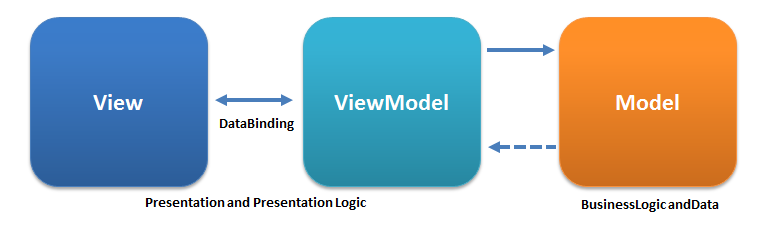
\includegraphics[width=\textwidth]{img/MVVMPattern.png}
        \caption{Three core components of the MVVM design pattern.}
        \label{fig:mvvm_pattern}
        %\source{https://en.wikipedia.org/wiki/Model%E2%80%93view%E2%80%93viewmodel#/media/File:MVVMPattern.png}
        \caption*{Source: \url{https://en.wikipedia.org/wiki/Model\%E2\%80\%93view\%E2\%80\%93viewmodel\#/media/File:MVVMPattern.png}}
    \end{figure}
    
    In the above graph \ref{fig:mvvm_pattern} relations between individual components are presented.
    
    \subsubsection{View}
        View in this case is a synonym of UI (in most cases GUI). Its purpose is to define the appearance of an app -- where and how do buttons look an lay, how the data is presented to the user, which elements are static and which have dynamic binding. As the name suggests, it handles the \textit{view} of the project - what user sees on the screen.
        
        In the presented application role of the \textit{View} part is taken by a project named \textit{View} \ref{fig:view}.
        
        \begin{figure}[H]
            \centering
            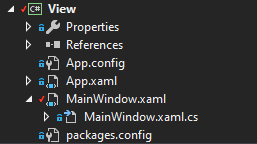
\includegraphics{img/view.png}
            \caption{\textit{View} project seen from Solution Explorer.}
            \label{fig:view}
        \end{figure}
        
        This project \ref{fig:view}, based on Visual Studio 2019 default project \textit{WPF App (.NET Framework)} \ref{fig:view_wpfApp} is the only non-F\# part of the MARS App as, for the time being (December 2020), there is no dedicated project in the F\# language that would, by default, be compatible with MVVM architecture and XAML markup language for presenting the view. Therefore few lines of C\# code needed to be added in order to bind successfully View project with ViewModel one.
        
        \begin{figure}
            \centering
            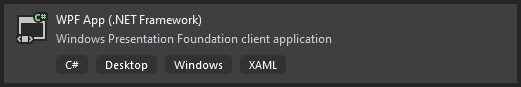
\includegraphics{img/view_wpfApp.png}
            \caption{Default Visual Studio 2019 project used for writing the \textit{View} part of an app.}
            \label{fig:view_wpfApp}
        \end{figure}

    \subsubsection{Model}
        \textit{Model} section handles business logic and data of the app. It is an inherent entity that could be reused in other applications. It is a significant advantage of the MVVM architectural pattern -- reusability of code is supported at the conceptual level of the design pattern.
        
        This time \textit{Model} project \ref{fig:model_VS19Project} is solely an F\# project that targets .Net Framework 4.6.1.
        \begin{figure}[H]
            \centering
            
\includegraphics{img/model_VS19Project.png}
            \caption{Default Visual Studio 2019 project used for writing the \textit{Model} part of an app.}
            \label{fig:model_VS19Project}
        \end{figure}
        
        In here it is useful to remind that whenever there is no valid reason to use \textit{.NET Core} over \textit{.NET Framework}, one should always opt for the latter. \textit{.NET Core} is used when multi-platform approach is expected, but if the app is destined for Microsoft Windows system then, the amount of libraries available on \textit{.NET Standard} is vastly higher.
        
        \begin{figure}[H]
            \centering
            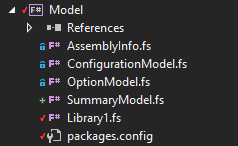
\includegraphics{img/model.png}
            \caption{\textit{Model} project seen from Solution Explorer.}
            \label{fig:model}
        \end{figure} 
        
    \subsubsection{ViewModel}    
        Last but surely not least the \textit{ViewModel} serves a role of a so-called \textit{bridge} between \textit{View} and the \textit{Model}. It binds the graphical presentation of the components with hidden back-end logic. It must hold a reference to the \textit{Model} project of the solution. It is extremely important for the programmer to design proper updates of data presented in corresponding graphic fields. \textit{INotifyPropertyChanged} interface is perfect for this purpose. It makes sure no change in the data filed will go unnoticed if it is able to see it anywhere in the app by the user.
        
        It consists of multiple files responsible for specific purposes, all starting with line:
        
        \begin{lstlisting}[language=FSharp, label={lst:model1}, caption=F\# all \textit{ViewModel} project components beginning.]
            namespace ViewModel
            // lines of code
        \end{lstlisting}
        
        Alternative syntax could be using F\# \textit{module} declaration what is rather more common nowadays that OOP-resembling \textit{namespace} like so:
        
        \begin{lstlisting}[language=FSharp, label={lst:model2}, caption=F\# alternative example \textit{ViewModel} project component beginning.]
            module MARSApp.ViewModel.ConfigurationViewModel
            open MARSApp.ViewModel.ViewModelBase
            open MARSApp.Model.ConfigurationModel
            // lines of code
        \end{lstlisting}
        
        Although the difference and these code fragments \ref{lst:model1} \ref{lst:model2} may seem unimportant, there is a tremendous reason behind choosing the first one -- since the project contains GUI written in XAML there is need to specify in the view where certain properties can be found. It turns out there is a major problem if the properties lay hidden inside a module. When they are presented in a namespace it is easier to bind them with XAML as it is adapted to receive a \textit{namespace} declaration in the \textit{Window} heading:
        
        \begin{figure}[H]
            \centering
            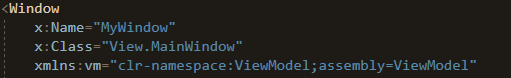
\includegraphics{img/viewmodel_namespace.png}
            \caption{Fragment of file \textit{MainWindow.xaml} showing \textit{namespace} reference.}
            \label{fig:viewmodel_namespace}
        \end{figure}
        
        The reference would be much harder to achieve if \textit{module} approach was used.
        
        For the sake of implementing \textit{ViewModel} in this example the same default VS19 project was used as in \textit{Model} project.
        
        \begin{figure}[H]
            \centering
            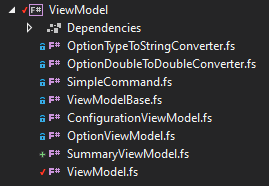
\includegraphics{img/viewmodel.png}
            \caption{\textit{ViewModel} project seen from Solution Explorer.}
            \label{fig:viewmodel}
        \end{figure} 
    
\subsection{XAML}
    \textit{XAML} stands for Extensible Application Markup Language and belongs to declarative markup language group. It is used in \textit{WPF} (\textit{Windows Presentation Forms} -- User Interface framework for creating desktop client applications \cite{wpf}) for separating between how an application looks like and how it behaves \cite{how_xaml_works} (both the GUI and its behavior were created in the same language). \textit{XAML} is an subset of \textit{XML}, because every \textit{XAML} file is as well a \textit{XML} file, but not every \textit{XML} file is a \textit{XAML} file.
    
    \textit{XAML} may resemble \textit{HTML}, although the idea behind those two is utterly different -- by comparing \textit{XML} to \textit{HTML} one can observe that:
    \begin{itemize}
        \item \textit{XML} is a markup language much like \textit{HTML} but \textit{HTML} was designed to display data while \textit{XML} to carry it.
        \item \textit{HTML} tags (such as: <p>, <h1>, <table>, etc.) are predefined while \textit{XML} ones are created at the moment by the programmer.
        \item \textit{HTML} allows small coding errors and is case insensitive in opposition to \textit{XML}.
    \end{itemize}

\chapter{Application}
\section{Theoretical background}

\subsection{Geometric Brownian Motion}
\todo
it's basically Wiener Process\^2

\subsection{Options}
    Options are some of the most popular derivative financial instruments. Derivative means in this example that it's value is reliant upon an underlying asset. The most important thing about options, one that distinguishes them from other derivative instruments it the \textbf{optionality} -- contract can, be is not obligatory to be made.
    
    There are 2 main types of options:
    \begin{itemize}
        \item \textbf{Call option} -- the buyer of the call option earns a right (not an obligation) to exercise his option to buy a particular asset from the call option seller for a stipulated period of time,
        \item \textbf{Put option} -- the buyer of the put option earns a right to exercise his option to sell a particular asset to the put option seller for a stipulated period of time\cite{Call_Put_Option_Definition}.
    \end{itemize}
    
    There are several parameters that describe an option, most important ones are:
    \begin{itemize}
        \item \textbf{Expiration Date} -- Specific moment in time by which the holder of the option has to decide whether he wants to exercise (use) the option.
        \item \textbf{Strike Price} -- agreed price at which the derivative underlying asset can be bought or sold (depends on a type of option) when it is exercised.
    \end{itemize}
    
    Further division into option types depends on when the option can be exercised. The most basic one is \textbf{European}-style option -- decision whether option will or will not be exercised is made at the time of option's expiry. Continuous option type is an \textbf{American} option -- option can be exercised at any time before the expiry. Combination of those two can be found in \textbf{Burmudan} Option -- contract can be exercised at specific days before the expiration. In this paper European Options will be presented\cite{Option_Types}.

\subsection{Black-Scholes Model}
    The Black--Scholes (or also called Black--Scholes--Merton) formula was created back in 1970s by 3 major economists: Fischer Black, Myron Scholes and Robert Merton (Scholes and Merton were awarded Nobel prize for economics in 1997. Certainly same would happen for Black if sadly it was not for his death in 1975).
    
    Their model was a significant breakthrough in world of mathematical models used for pricing derivative instruments. It provides a framework for European-style option valuations, such as calls and puts.
    
    This thesis' aim was not to goo deep into understanding the mathematical background behind the model but rather implement the model in a practical tool that one would be able to effectively use. Therefore more information and specifics can be found either in the original publication \cite{10.2307/1831029} of the model from 1973 in \textit{The Pricing of Options and Corporate Liabilities} of the Journal of Political Economy by Fischer Black and Myron Scholes.
    
    Main formula of the model used for option pricing is as follows:
    $$
    C = S_0\phi(d_1) - Ke^{-rT}\phi(d_2)
    $$
    $$
    P = -S_0\phi(-d_1) + Ke^{-rT}\phi(-d_2)
    $$
    $$
    d_1 = ln\frac{S_0}{K} + (r+\frac{\sigma^2}{2})t
    $$
    $$
    d_2 = d_1 - \sigma\sqrt{t},
    $$
    where:
    \begin{itemize}
        \item $C$ - call option price
        \item $P$ - put option price
        \item $S_0$ - underlying asset price at the time being
        \item $\phi()$ - standardized cumulative normal distribution
        \item $K$ - strike price
        \item $r$ - risk free rate (1\% represented as 0.01)
        \item $t$ - time to maturity in years (18 months represented as 1.5)
        \item $\sigma$ - volatility (20\% represented as 0.2)
    
    \end{itemize}
    
    The formula assumes that the price history of an underlying asset (in this example - a stock price) has a lognormal distribution and follows geometric Brownian motion with constant drift and volatility. 
    \todo{diff eq thats at the core of the model as curiosity}
\chapter{Conclusions}
\section{Have the assumptions been met?}
    In conclusion, the aim of this thesis has been achieved by creating a program -- \textit{MARS App} -- that fulfills this work's assumptions. 83\% of the code behind the app is an F\# code and, wherever possible, functional approach was used. Therefore, the functional part is covered without a doubt.
    
    Subsequently, derivative financial instrument in the form of a European-style option has been implemented and priced under the \textit{Black-Scholes Model} as presented in fig. \ref{fig:optionsPresentation}. Underlying asset's history has been generated using \textit{Geometric Brownian Motion}, as presented in the previous chapter. Ability to specialize the product has been introduced as well, what can bee seen in the fig. \ref{fig:parametersPresentation}. Elements of the graphic design concerning product specialization, option presentation and \textit{GBM} visualisation can be seen in corresponding sections.
    
    This way all assumptions have been met and several conclusions can be drawn from this work:
    \begin{itemize}
        \item Complex mathematical models can be introduced in few lines of F\# code.
        \item For the time being (December 2020) F\# language is not the best choice for creating a desktop application due to not large enough community, lack of tutorials and overall onerousness related to binding UI with back-end logic.
        \item \textit{Black--Scholes Model}, although nearly 50-year-old, is still widely used despite the era of Artificial Intelligence and its benefits.
    \end{itemize}
    
\section{Further development possibilities}
    Future works may concern adding:
    \begin{itemize}

        \item connection to an online database in order to use historical data for an underlying asset instead of artificial trends generated by \textit{GBM},
        \item so-called \textit{greeks} to further improve \textit{MARS App} utility,
        \item \textit{Monte Carlo Simulation} (written in C++ to speed up computing) as another model for comparison with \textit{GBM}.
    \end{itemize}
\include{chapter04}
\include{chapter05}
\include{chapter06}

% wstawię tutaj, czy spis rysunkow przeniesie się na koniec?
%   > tak!
\newpage
\mbox{}\pdfbookmark[0]{List of figures}{spisRysunkow.1}
\addcontentsline{toc}{chapter}{List of figures}
\listoffigures*


% \bibliographystyle{plalpha}
\bibliographystyle{abbrv}
% \bibliographystyle{plain}

%Warning: References should be collected in a separate file. You can use the programm JabRef for editing. 
%         But please remember, that not all JabRef types of entries are supported by BibTeX.
%         File name below is given without extenion 
%         (here BibTeX will look for "bibiography.bib" in the main directory)
\setlength{\bibitemsep}{2pt} % introduced to make smaller seps between bibliographic items
\bibliography{bibliography}
\appendix
\chapter{CD/DVD included}
% \section{CD/DVD included}
Included CD/DVD contains the following directories:

\dirtree{%
.1 /.
.2 MARS\_App \ldots{}
\begin{minipage}[t]{8cm}
    This directory holds entire projects that create the solution as well as \textit{{.}sln} file for easy further development in Microsoft Visual Studio 2019{.}
\end{minipage}.
.2 thesis\_pdf \ldots{} 
\begin{minipage}[t]{8cm}
    This directory contains \textit{{.}pdf} version of the Engineering Thesis{.}
\end{minipage}.
}
\include{appendixB}

%%Uncomment the lines below, if you want to use index
%%\chapterstyle{noNumbered}
%%\phantomsection 
%%\addcontentsline{toc}{chapter}{Index}
%%\printindex

\end{document}